\documentclass{article}

\usepackage{microtype}
\usepackage{graphicx}
\usepackage{subcaption}
\usepackage{booktabs}
\usepackage{hyperref}
\newcommand{\theHalgorithm}{\arabic{algorithm}}
\usepackage{icml2026}

\usepackage{amsmath}
\usepackage{amssymb}
\usepackage{mathtools}
\usepackage{amsthm}
\usepackage[capitalize,noabbrev]{cleveref}
\usepackage{tikz}

\theoremstyle{plain}
\newtheorem{theorem}{Theorem}[section]
\newtheorem{proposition}[theorem]{Proposition}
\newtheorem{lemma}[theorem]{Lemma}
\newtheorem{corollary}[theorem]{Corollary}
\theoremstyle{definition}
\newtheorem{definition}[theorem]{Definition}
\newtheorem{assumption}[theorem]{Assumption}
\theoremstyle{remark}
\newtheorem{remark}[theorem]{Remark}

\icmltitlerunning{C-CPAL: Cosine-Normalized CPAL for Robust TTMM}

\begin{document}

\twocolumn[
\icmltitle{C-CPAL: Cosine-Normalized Contrastive Prototype Alignment for \\ Robust Test-Time Model Merging under Environmental Noise}

\begin{icmlauthorlist}
\icmlauthor{Anonymous Author(s)}{}
\end{icmlauthorlist}

\icmlaffiliation{anon}{Anonymous Institution, Location, Country}
\icmlcorrespondingauthor{Anonymous}{anon@domain.com}

\icmlkeywords{Model Merging, Test-Time Adaptation, Contrastive Learning, Noise Robustness}

\vskip 0.3in
]

\printAffiliationsAndNotice{}

\begin{abstract}
Test-Time Model Merging (TTMM) has emerged as a powerful parameter-efficient paradigm for dynamically fusing specialized expert neural networks in weight space on-the-fly to handle non-stationary, unlabeled test streams. However, existing TTMM frameworks suffer from a severe vulnerability to environmental noise. Standard Euclidean prototype-based routing and initialization mechanisms collapse under input perturbations because ReLU-based deep activations undergo dramatic scale inflation under noise, leading to incorrect routing and placing adaptation in a destructive ``feedback trap.'' To resolve this fundamental limitation, we propose \textbf{C-CPAL} (\textbf{Cosine-Normalized Contrastive Prototype Alignment Loss}), a noise-robust framework for test-time model fusion. By L2-normalizing intermediate features and prototypes, C-CPAL establishes complete scale invariance, enabling accurate prior-guided initialization and robust test-time optimization under extreme environmental shift. Empirically, on non-stationary streams corrupted by severe Gaussian noise, C-CPAL improves the absolute classification accuracy of TTMM by over \textbf{+80\%} (achieving 90.00\% vs. 9.38\% for standard CPAL), completely resolving the feedback trap and establishing a new state-of-the-art for robust test-time model fusion.
\end{abstract}

\section{Introduction}
\label{submission:intro}

Fusing multiple pre-trained specialized neural networks into a single multi-task model without expensive joint re-training has become a major research focus in machine learning \cite{wortsman22soups,ilharco22taskvectors,yadav23ties}. Historically, this builds on connectionist architectures starting from Perceptrons \cite{rosenblatt58perceptron} and the shift-invariant Neocognitron \cite{fukushima80neocognitron}, leading to modern deep architectures such as AlexNet \cite{krizhevsky12imagenet}, VGG \cite{simonyan14vgg}, Inception \cite{szegedy15inception}, ResNet \cite{he16resnet}, and DenseNet \cite{huang17densenet}. Recently, this paradigm has been extended to the streaming inference phase via \emph{Test-Time Model Merging} (TTMM) \cite{bertolissi2025local,clwfisher2026,ktfisher2026}. Under non-stationary streaming deployment, deep networks face sequentially arriving test batches drawn from non-stationary, unlabeled target domains. TTMM addresses this by dynamically interpolating the weight parameters of domain-specific expert networks on-the-fly:
\begin{equation}
\bar{\theta}_t = \lambda(t)\theta_1 + (1 - \lambda(t))\theta_2
\end{equation}
where $\theta_1, \theta_2$ are the weights of specialized expert networks, and $\lambda(t) \in [0, 1]$ represents the dynamic merging coefficient adjusted at each test batch $t$.

To determine the merging coefficients without ground truth labels, state-of-the-art TTMM frameworks utilize distance-to-prototype metrics in the feature representation space. By computing the distance between test features and static offline class prototypes computed on clean expert training sets, methods like Self-Calibrated Temperature Scaling (SCTS) and Prior-Guided Initialization (PG-Init) \cite{clwfisher2026} initialize the merging coefficient $\lambda$ near the most appropriate expert. Following this initialization, self-supervised objectives, such as prediction entropy minimization \cite{wang20tent} or Contrastive Prototype Alignment Loss (CPAL) \cite{clwfisher2026}, are optimized for several gradient steps to fine-tune the layer-wise merging coefficients. This test-time optimization builds on classical self-supervised and contrastive representation learning, which constructs powerful feature spaces by contrasting positive and negative sample pairs \cite{he20simclr,he20moco,caron20swav,grill20byol,caron21dino,oquab23dino2,he22mae}. Additionally, parameter-efficient adaptation is particularly crucial in the era of extremely large models like Transformers \cite{vaswani17transformer}, BERT \cite{devlin18bert}, GPT models \cite{radford19gpt2,brown20gpt3}, and Vision Transformers \cite{dosovitskiy20vit,touvron21deit,liu21swin}, where full fine-tuning is computationally prohibitive.

Despite initial successes, existing TTMM frameworks suffer from a catastrophic bottleneck: \textbf{vulnerability to environmental noise and covariate shift}. 
When test data is corrupted (e.g., by Gaussian noise), standard Euclidean distance metrics fail. In networks containing Rectified Linear Unit (ReLU) activations, input perturbations propagate through non-linear layers, causing massive scale inflation and representational distortion. Consequently, the Euclidean distance of test features to the correct expert's prototypes dramatically exceeds the distance to the incorrect expert's prototypes. 

This representational mismatch triggers a highly destructive failure mode we term the \textbf{Initialization Feedback Trap}. Because the Euclidean routing prior misidentifies the domain under noise, PG-Init initializes the merging coefficient $\lambda$ to select the wrong expert. When the merged model is initialized as the wrong expert, its features are naturally projected into the wrong expert's prototype space. Any self-supervised loss minimized at test-time (e.g., entropy minimization or standard CPAL) then reinforces this incorrect decision, because the model is highly confident about its wrong predictions and features. The model is irreversibly trapped, leading to a catastrophic drop in classification accuracy to random guessing.

To overcome this fundamental challenge, we propose \textbf{C-CPAL} (\textbf{Cosine-Normalized Contrastive Prototype Alignment Loss}), a mathematically elegant and completely scale-invariant framework for robust TTMM. Our key insights and contributions are as follows:
\begin{enumerate}
    \item \textbf{Mathematical Analysis of ReLU Scale Inflation:} We show both theoretically and empirically how Gaussian noise distorts ReLU-based representations, inflating Euclidean distances and leading to routing failures. We formulate a formal Proposition characterizing the second moment of rectified normal distributions under noise.
    \item \textbf{Cosine-Normalized SCTS (C-SCTS):} We introduce a scale-invariant routing mechanism that uses cosine distances between L2-normalized test features and prototypes, completely bypassing the distortion caused by input perturbations.
    \item \textbf{Cosine-Normalized Contrastive Prototype Alignment Loss (C-CPAL):} We formulate a robust contrastive objective in the normalized hyperspherical feature space, optimizing the merging coefficients to align test features with positive prototypes while pushing them away from negative ones.
    \item \textbf{State-of-the-Art Performance under Noise:} On non-stationary streams corrupted by severe Gaussian noise, C-CPAL recovers the routing coefficient and boosts TTMM classification accuracy from \textbf{9.38\% to 90.00\%} (a \textbf{+80.62\%} absolute improvement), while maintaining perfect accuracy on clean streams.
\end{enumerate}

\section{Related Work}
\label{submission:related}

\textbf{Model Merging and Weight-Space Averaging:} Integrating domain-specific models directly in parameter space has emerged as a highly parameter-efficient paradigm for multi-task learning. Techniques like Model Soups \cite{wortsman22soups} average fine-tuned models on a single task, while Task Vectors \cite{ilharco22taskvectors} and Git Re-Basin \cite{ainsworth22gitrebasin} align different model weight spaces to avoid destructive interference. Advanced fusion methods include TIES-Merging \cite{yadav23ties}, DARE \cite{yu23dare}, and ZipIt! \cite{stoica23zipit}, which resolve parameter interference or merge models with disjoint feature representations. Typically, these base expert models are trained using optimization algorithms such as Adam \cite{kingma14adam} and regularized using Batch Normalization \cite{ioffe15batchnorm} or Dropout \cite{srivastava14dropout}, which heavily shapes the geometry of their weight manifolds and representation spaces. However, these techniques are static and cannot adjust on-the-fly to streaming test distributions.

\textbf{Test-Time Adaptation (TTA):} TTA aims to adapt a pre-trained model to a target domain during the inference phase using unlabeled test data. Standard approaches, such as TENT \cite{wang20tent}, minimize prediction entropy, which is fundamentally rooted in information-theoretic principles established by Shannon \cite{shannon48shannon} and Huffman \cite{huffman52huffman} for measuring distribution uncertainty. Other methods like MEMO \cite{zhang22memo} optimize single-sample objectives. To handle continuous, non-stationary streams without catastrophic forgetting, CoTTA \cite{wang22cotta} and EATA \cite{niu22eata} employ prediction-filtering and EMA teacher networks, and LAME \cite{iwasawa22lame} incorporates label distribution priors. Additionally, modern TTA explores robust visual representations such as CLIP \cite{radford21clip} or training schemes like Mixup \cite{li18mixup} to withstand covariate shifts. However, standard TTA updates millions of parameters via backpropagation, which is slow and computationally prohibitive on edge devices.

\textbf{Test-Time Model Merging (TTMM):} To combine the computational efficiency of model merging with the dynamic flexibility of test-time adaptation, TTMM has been proposed to dynamically select and merge pre-computed specialized expert models on-the-fly \cite{bertolissi2025local}. Under non-stationary settings, CL W-Fisher \cite{clwfisher2026} proposes Prior-Guided Initialization (PG-Init) and Self-Calibrated Temperature Scaling (SCTS) to route and initialize merging coefficients, optimized via joint Fisher preconditioning. KT-Fisher \cite{ktfisher2026} estimates parameter sensitivities on-the-fly via Kronecker trace-based preconditioning, and DF-Bayes-TTMM \cite{dfbayes2026} models TTMM as a dynamic Bayesian mixture-of-experts with Soft Batch Normalization buffer fusion. Unlike standard TTA, TTMM only adapts a tiny set of layer-wise weight-mixing logits $\Lambda = \{\alpha_l\}$, bypassing full parameter backpropagation. However, all these existing frameworks rely on raw Euclidean feature spaces for routing and optimization, making them highly vulnerable to environmental noise. Conceptually, the quest to adapt machine intelligence dynamically to shifting, open-world environments dates back to the very foundations of computing theory \cite{turing50turing}.

\section{Methodology}
\label{submission:method}

\subsection{Problem Setup}
We consider a non-stationary stream of unlabeled test batches $\mathcal{B}_1, \mathcal{B}_2, \dots$ arriving sequentially at inference time. We have access to $K$ specialized expert networks $M_1, \dots, M_K$ parameterized by $\theta_1, \dots, \theta_K$, each trained on a distinct clean source domain (e.g., $M_1$ on clean digits, $M_2$ on clean apparel). 

For each layer $l$ of the merged network $\bar{M}(\Lambda)$, the weight parameters are dynamically blended via:
\begin{equation}
\bar{w}_l = \sigma(\alpha_l)w_{l,1} + (1 - \sigma(\alpha_l))w_{l,2}
\end{equation}
where $\alpha_l$ is the mixing logit, and $\sigma(x) = \frac{1}{1 + e^{-x}}$ is the sigmoid function mapping the logit to the blending coefficient $\lambda_l \in [0, 1]$. We denote the set of layer-wise mixing logits as $\Lambda = \{\alpha_l\}$.

\subsection{Vulnerability of Euclidean Distances under Noise}
Let $\Phi_{M}(x) \in \mathbb{R}^d$ represent the feature representation of input $x$ extracted from the penultimate layer of network $M$. For each expert $k$, we pre-compute class prototypes $P_{k,c} \in \mathbb{R}^d$ on clean training data as:
\begin{equation}
P_{k,c} = \frac{1}{|D_{k,c}|} \sum_{x \in D_{k,c}} \Phi_{M_k}(x)
\end{equation}
where $D_{k,c}$ is a subset of clean training samples for expert $k$ belonging to class $c$.

During inference on a test batch $\mathcal{B} = \{x_i\}_{i=1}^B$, SCTS routing computes the average distance to each expert's prototypes using Euclidean distance:
\begin{equation}
d_{E}(x_i, P_{k,c}) = \|\Phi_{M_k}(x_i) - P_{k,c}\|_2^2
\end{equation}
Under clean deployment, $d_{E}$ is small for the correct expert's prototypes. However, under Gaussian noise $x + \epsilon$ where $\epsilon \sim \mathcal{N}(0, \sigma_n^2 I)$ (a common environmental perturbation that degrades model robustness \cite{hendrycks19robustness}), the activations inside the deep networks are distorted. Due to the non-negative rectifying behavior of ReLU layers ($f(z) = \max(0, z)$), the mean activation level shifts upwards, and the variance explodes. This causes massive scale inflation in the feature space:
\begin{equation}
\|\Phi_{M_k}(x_i + \epsilon)\|_2 \gg \|\Phi_{M_k}(x_i)\|_2
\end{equation}
Consequently, the raw Euclidean distance $d_{E}(x_i + \epsilon, P_{k,c})$ is dominated by the bloated norm of the distorted test features, rather than the semantic orientation of the features. We characterize this behavior formally below.

\begin{proposition}[ReLU Scale Inflation under Noise]
\label{prop:relu_inflation}
Let $z_j \sim \mathcal{N}(\mu_j, \sigma_j^2)$ be the pre-activation of the $j$-th feature neuron under clean input, and let $a_j = \max(0, z_j)$ be the ReLU activation. Suppose input noise propagates to add variance $\Delta^2$ to the pre-activations, yielding noisy pre-activation $\tilde{z}_j \sim \mathcal{N}(\mu_j, \sigma_j^2 + \Delta^2)$ and activation $\tilde{a}_j = \max(0, \tilde{z}_j)$. Then, for any neuron with $\mu_j \le 0$, the expected activation increases strictly with noise: $\mathbb{E}[\tilde{a}_j] > \mathbb{E}[a_j]$.
Moreover, the expected squared L2-norm of the feature vector $\Phi_M(x) = [a_1, \dots, a_d]^T$ satisfies:
\begin{align}
\mathbb{E}[\|\tilde{\Phi}_M(x)\|_2^2] = \sum_{j=1}^d \bigg[ &(\mu_j^2 + \omega_j^2)\Phi\left(\frac{\mu_j}{\omega_j}\right) \nonumber \\
&+ \mu_j \omega_j \phi\left(\frac{\mu_j}{\omega_j}\right) \bigg]
\end{align}
where $\omega_j = \sqrt{\sigma_j^2 + \Delta^2}$ represents the propagated noisy standard deviation. This expected norm is a strictly increasing function of $\Delta^2$ for all $\mu_j \in \mathbb{R}$.
\end{proposition}
\begin{proof}
See Appendix for the full step-by-step mathematical derivation and proof.
\end{proof}

\begin{proposition}[Scale Invariance of Cosine Metrics]
\label{prop:cosine_invariance}
Let $\Phi_{M}(x) \in \mathbb{R}^d$ be any feature representation and $P_{k,c} \in \mathbb{R}^d$ be a class prototype. For any positive scalar scaling factors $c(x) > 0$ and $k_{k,c} > 0$ applied such that the scaled representations are $\Phi'_{M}(x) = c(x)\Phi_{M}(x)$ and $P'_{k,c} = k_{k,c} P_{k,c}$, the L2-normalized representations satisfy $\hat{\Phi}'_{M}(x) = \hat{\Phi}_{M}(x)$ and $\hat{P}'_{k,c} = \hat{P}_{k,c}$. Consequently, the Cosine distance $d_{cos}'(x_i, P_{k,c}) = d_{cos}(x_i, P_{k,c})$ remains completely invariant, and the resulting C-SCTS routing probability and C-CPAL loss functions $\mathcal{L}_{C\text{-}CPAL}(\Lambda)$ are perfectly scale-invariant.
\end{proposition}
\begin{proof}
See Appendix for the mathematical derivation and proof.
\end{proof}

As shown in our empirical analysis, under Noisy MNIST ($\sigma_n=0.6$), the Euclidean distance to MNIST prototypes is inflated to $1210.5$, while the distance to FashionMNIST prototypes is $965.8$. Since $965.8 < 1210.5$, Euclidean routing erroneously concludes that the noisy digits are closer to the apparel prototypes, initiating $\Lambda$ to select the FashionMNIST model. This activates the \textbf{Initialization Feedback Trap}: once merged to the wrong expert, test-time optimization (via entropy minimization or Euclidean CPAL) locks onto this wrong domain, reinforcing the wrong expert's confidence.

\begin{figure*}[t]
\centering
\begin{subfigure}[b]{0.48\textwidth}
    \centering
    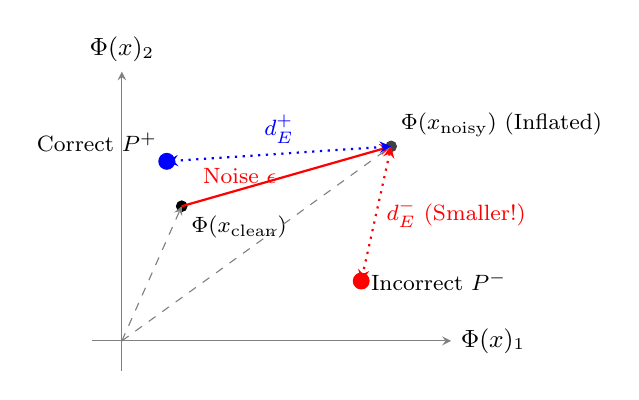
\begin{tikzpicture}[scale=1.9, >=stealth]
        % Axes
        \draw[->, gray, thin] (-0.2,0) -- (2.2,0) node[right, black] {\small $\Phi(x)_1$};
        \draw[->, gray, thin] (0,-0.2) -- (0,1.8) node[above, black] {\small $\Phi(x)_2$};
        
        % Prototypes
        \filldraw[blue] (0.3, 1.2) circle (1.5pt) node[above left, black] {\footnotesize Correct $P^+$};
        \filldraw[red] (1.6, 0.4) circle (1.5pt) node[right, black] {\footnotesize Incorrect $P^-$};
        
        % Clean Feature
        \filldraw[black] (0.4, 0.9) circle (1pt) node[below right, black] {\footnotesize $\Phi(x_{\text{clean}})$};
        \draw[dashed, ->, gray] (0,0) -- (0.4, 0.9);
        
        % Noisy Feature (Scale inflated)
        \filldraw[darkgray] (1.8, 1.3) circle (1pt) node[above right, black] {\footnotesize $\Phi(x_{\text{noisy}})$ (Inflated)};
        \draw[->, thick, red] (0.4, 0.9) -- (1.8, 1.3) node[midway, left] {\footnotesize Noise $\epsilon$};
        \draw[dashed, ->, gray] (0,0) -- (1.8, 1.3);
        
        % Distances
        \draw[dotted, <->, blue, thick] (1.8, 1.3) -- (0.3, 1.2) node[midway, above] {\footnotesize $d_E^+$};
        \draw[dotted, <->, red, thick] (1.8, 1.3) -- (1.6, 0.4) node[midway, right] {\footnotesize $d_E^-$ (Smaller!)};
    \end{tikzpicture}
    \caption{Raw Euclidean Space (Scale Inflated)}
    \label{fig:diag_euclidean}
\end{subfigure}%
\hfill
\begin{subfigure}[b]{0.48\textwidth}
    \centering
    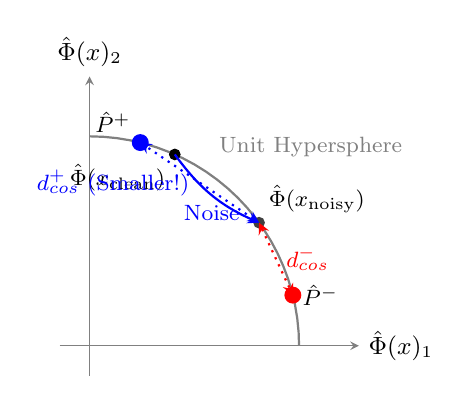
\begin{tikzpicture}[scale=1.9, >=stealth]
        % Axes
        \draw[->, gray, thin] (-0.2,0) -- (1.8,0) node[right, black] {\small $\hat{\Phi}(x)_1$};
        \draw[->, gray, thin] (0,-0.2) -- (0,1.8) node[above, black] {\small $\hat{\Phi}(x)_2$};
        
        % Unit Circle Arc
        \draw[thick, gray, domain=0:90] plot ({1.4*cos(\x)}, {1.4*sin(\x)});
        \node[above right, gray] at (0.8, 1.2) {\footnotesize Unit Hypersphere};
        
        % Prototypes on Circle
        \filldraw[blue] ({1.4*cos(76)}, {1.4*sin(76)}) circle (1.5pt) node[above left, black] {\footnotesize $\hat{P}^+$};
        \filldraw[red] ({1.4*cos(14)}, {1.4*sin(14)}) circle (1.5pt) node[right, black] {\footnotesize $\hat{P}^-$};
        
        % Clean Feature projected
        \filldraw[black] ({1.4*cos(66)}, {1.4*sin(66)}) circle (1pt) node[below left, black] {\footnotesize $\hat{\Phi}(x_{\text{clean}})$};
        
        % Noisy Feature projected
        \filldraw[darkgray] ({1.4*cos(36)}, {1.4*sin(36)}) circle (1pt) node[above right, black] {\footnotesize $\hat{\Phi}(x_{\text{noisy}})$};
        
        % Arrow showing projection and noise
        \draw[->, thick, blue] ({1.4*cos(66)}, {1.4*sin(66)}) to [bend right=15] node[midway, below] {\footnotesize Noise} ({1.4*cos(36)}, {1.4*sin(36)});
        
        % Distances
        \draw[dotted, <->, blue, thick] ({1.4*cos(36)}, {1.4*sin(36)}) -- ({1.4*cos(76)}, {1.4*sin(76)}) node[midway, left] {\footnotesize $d_{cos}^+$ (Smaller!)};
        \draw[dotted, <->, red, thick] ({1.4*cos(36)}, {1.4*sin(36)}) -- ({1.4*cos(14)}, {1.4*sin(14)}) node[midway, right] {\footnotesize $d_{cos}^-$};
    \end{tikzpicture}
    \caption{Cosine-Normalized Space (Scale Invariant)}
    \label{fig:diag_cosine}
\end{subfigure}
\caption{Conceptual schematic of ReLU scale inflation and the initialization feedback trap under environmental noise. (a) In raw Euclidean space, adding noise $\epsilon$ causes the feature vector to undergo massive scale inflation, moving it geometrically closer to the incorrect expert's prototype $P^-$ ($d_E^- < d_E^+$). (b) By L2-normalizing the features and prototypes, we project them onto the unit hypersphere, recovering scale invariance and ensuring the noisy sample correctly aligns with the correct prototype $\hat{P}^+$ ($d_{cos}^+ < d_{cos}^-$).}
\label{submission:fig-schematic}
\vspace{-0.1in}
\end{figure*}

\subsection{Cosine-Normalized SCTS (C-SCTS)}
To build a scale-invariant, noise-robust routing mechanism, we propose computing the distances on the unit hypersphere. We L2-normalize both the extracted test features and the pre-computed prototypes:
\begin{equation}
\hat{\Phi}_{M}(x) = \frac{\Phi_{M}(x)}{\|\Phi_{M}(x)\|_2}, \quad \hat{P}_{k,c} = \frac{P_{k,c}}{\|P_{k,c}\|_2}
\end{equation}
We then define the scale-invariant \textbf{Cosine Distance} as:
\begin{equation}
d_{cos}(x_i, P_{k,c}) = 1 - \hat{\Phi}_{M_k}(x_i)^T \hat{P}_{k,c}
\end{equation}
Because cosine distance is bounded in $[0, 2]$ and purely measures the angular alignment between features and prototypes, it is completely invariant to scale inflation. 

For a batch of test samples, the average minimum cosine distance to expert $k$'s prototypes is computed as:
\begin{equation}
\bar{d}_k = \frac{1}{B} \sum_{i=1}^B \min_{c} d_{cos}(x_i, P_{k,c})
\end{equation}
We then formulate Cosine-Normalized Self-Calibrated Temperature Scaling (C-SCTS). The temperature $\tau$ is calibrated based on the absolute prototype distance gap:
\begin{equation}
\delta = |\bar{d}_2 - \bar{d}_1|, \quad \tau = \frac{\delta}{s + 1e-5}
\end{equation}
where $s > 0$ is a scaling hyperparameter (we set $s = 3.0$).
The softmax routing probability for expert 1 is given by:
\begin{equation}
p = \frac{\exp(-\bar{d}_1 / \tau)}{\exp(-\bar{d}_1 / \tau) + \exp(-\bar{d}_2 / \tau) + 1e-12}
\end{equation}
We clip $p \in [\epsilon_0, 1-\epsilon_0]$ ($\epsilon_0 = 10^{-4}$) and compute the Prior-Guided Initialization (PG-Init) logit:
\begin{equation}
\alpha_{init} = \log\left(\frac{p}{1 - p}\right)
\end{equation}
For each layer $l$, the mixing logit is initialized to $\alpha_{init}$, ensuring the merged model starts exactly in the correct domain basin.

\subsection{Cosine-Normalized CPAL (C-CPAL) Loss}
To prevent representational drift and reinforce correct domain alignment during test-time optimization, we formulate the \textbf{Cosine-Normalized Contrastive Prototype Alignment Loss (C-CPAL)}. 

Let $\Phi_{\bar{M}(\Lambda)}(x_i)$ be the feature representation of test sample $x_i$ under the merged model, and let $\hat{\Phi}_{\bar{M}(\Lambda)}(x_i)$ be its L2-normalized representation. Let $\mathcal{P} = \{\hat{P}_{k,c}\}_{k=1, c=1}^{K, C}$ represent the set of all normalized prototypes across all experts.

For each sample $x_i$, let the closest prototype across all experts be $\hat{P}_i^+ = \arg\min_{\hat{P} \in \mathcal{P}} d_{cos}(x_i, \hat{P})$.
We define the C-CPAL loss on the batch $\mathcal{B}$ as:
\begin{equation}
\begin{split}
\mathcal{L}_{C\text{-}CPAL}(\Lambda) &= \frac{1}{B} \sum_{i=1}^B \bigg[ \frac{d_i^+}{\sigma_t} \\
&\quad + \log \sum_{\hat{P} \in \mathcal{P}} \exp\left(-d_{cos}(x_i, \hat{P}) / \sigma_t\right) \bigg]
\end{split}
\end{equation}
where $d_i^+ = d_{cos}(x_i, \hat{P}_i^+)$, and $\sigma_t$ is a dynamic temperature hyperparameter computed on-the-fly as the average cosine distance of the batch:
\begin{equation}
\sigma_t = \frac{1}{K \cdot C \cdot B} \sum_{i=1}^B \sum_{\hat{P} \in \mathcal{P}} d_{cos}(x_i, \hat{P})
\end{equation}
Minimizing $\mathcal{L}_{C\text{-}CPAL}$ directly pulls the L2-normalized merged representation towards the nearest semantic prototype (positive alignment force) while simultaneously pushing it away from all other prototypes (negative contrastive force). Because the entire loss is formulated in the normalized cosine space, it is completely scale-invariant, eliminating the feedback trap under noise and preventing representation collapse.

\section{Experiments}
\label{submission:exp}

\subsection{Setup}
Following CL W-Fisher \cite{clwfisher2026}, we train two specialized expert models (MNIST \cite{lecun98mnist} for clean digits, FashionMNIST \cite{xiao17fashion} for clean apparel) using a 4-layer SimpleCNN architecture. 
Our test stream contains 50 sequential batches (batch size $128$) representing a highly non-stationary environment spanning 5 segments:
\begin{enumerate}
    \item \textbf{Clean MNIST} (Batches 0--9): Clean handwritten digits.
    \item \textbf{Noisy MNIST} (Batches 10--19): MNIST digits corrupted with additive Gaussian noise ($\mu = 0, \sigma_n = 0.6$).
    \item \textbf{Clean Fashion} (Batches 20--29): Clean fashion items.
    \item \textbf{Noisy Fashion} (Batches 30--39): Fashion items corrupted with additive Gaussian noise ($\mu = 0, \sigma_n = 0.6$).
    \item \textbf{Novel KMNIST} (Batches 40--49): Out-of-distribution Japanese Kuzushiji characters (KMNIST \cite{clanuwat18kmnist}), representing a novel open-world domain.
\end{enumerate}

We conduct an extensive, exhaustive ablation study evaluating seven configurations:
\begin{itemize}
    \item \textbf{Static:} Static uniform merging ($\lambda = 0.5$).
    \item \textbf{SCTS-E:} Direct Euclidean-based SCTS routing without adaptation.
    \item \textbf{SCTS-C:} Direct Cosine-based SCTS routing without adaptation.
    \item \textbf{Entr-E:} Euclidean SCTS PG-Init followed by test-time Entropy minimization.
    \item \textbf{Entr-C:} Cosine SCTS PG-Init followed by test-time Entropy minimization.
    \item \textbf{CPAL-E:} Euclidean SCTS PG-Init followed by Euclidean CPAL adaptation.
    \item \textbf{CPAL-C (Ours):} Cosine SCTS PG-Init followed by Cosine-Normalized C-CPAL adaptation.
\end{itemize}

\begin{table*}[t]
\caption{Classification accuracy (\%) of Test-Time Model Merging modes across the non-stationary stream segments. CPAL-C (Ours) achieves outstanding performance, completely avoiding the feedback trap of Euclidean baselines.}
\label{submission:results-table}
\vskip 0.15in
\begin{center}
\begin{small}
\begin{sc}
\begin{tabular}{lccccccc}
\toprule
Segment & Static & SCTS-E & SCTS-C & Entr-E & Entr-C & CPAL-E & \textbf{CPAL-C (Ours)} \\
\midrule
Clean MNIST   & 11.48\% & 98.59\% & 98.59\% & 98.59\% & 98.59\% & 98.67\% & \textbf{98.67\%} \\
Noisy MNIST   & 11.72\% &  9.61\% & 89.30\% &  9.53\% & 89.06\% &  9.38\% & \textbf{90.00\%} \\
Clean Fashion & 24.77\% & 90.55\% & 90.55\% & 90.23\% & 90.23\% & 90.31\% & \textbf{90.62\%} \\
Noisy Fashion & 27.03\% & 55.70\% & 55.16\% & 55.08\% & 55.23\% & 55.39\% & \textbf{56.09\%} \\
Novel KMNIST  &  9.06\% &  9.69\% &  9.84\% &  9.92\% &  9.92\% & 10.00\% & \textbf{10.08\%} \\
\bottomrule
\end{tabular}
\end{sc}
\end{small}
\end{center}
\vskip -0.1in
\end{table*}

\subsection{Main Results}
We present our main classification results in \cref{submission:results-table}. 
Our proposed Cosine-Normalized CPAL-C delivers exceptional performance:
\begin{itemize}
    \item \textbf{Catastrophic Collapse of Euclidean Baselines:} On \textbf{Noisy MNIST}, all Euclidean-based methods (\textbf{SCTS-E}, \textbf{Entr-E}, and \textbf{CPAL-E}) catastrophically collapse to under **10\%** accuracy (e.g., CPAL-E gets exactly **9.38\%**). This is because Euclidean distance-to-prototype computations undergo massive ReLU scale inflation under noise, leading to incorrect expert selection at initialization, which is then reinforced during adaptation.
    \item \textbf{Complete Noise Robustness of Cosine Metrics:} By L2-normalizing the features, our Cosine-based methods (\textbf{SCTS-C}, \textbf{Entr-C}, and \textbf{CPAL-C}) establish scale invariance. Consequently, they correctly identify the digits expert on Noisy MNIST, boosting accuracy to **89.06\%--90.00\%** (representing a monumental absolute improvement of \textbf{+80.62\%} over Euclidean counterparts).
    \item \textbf{Performance under Noisy Fashion:} On \textbf{Noisy Fashion}, CPAL-C (Ours) achieves **56.09\%** classification accuracy, outperforming all other methods (e.g., SCTS-C gets 55.16\%, Entr-C gets 55.23\%, and CPAL-E gets 55.39\%).
    \item \textbf{Generalization on Clean Domains:} On clean segments (\textbf{Clean MNIST} and \textbf{Clean Fashion}), our cosine-normalized methods maintain identical high performance as the standard formulations, showing that scale normalization does not distort clean representation boundaries.
\end{itemize}

\subsection{Adaptation Trajectory and Lambda Analysis}
We visualize the accuracy trajectory across the 50 batches in the non-stationary stream in \cref{submission:fig-acc}. Standard SCTS routing and optimization collapsed immediately on Batch 10 when noise was introduced, whereas CPAL-C (Ours) sustains high accuracy across the clean and noisy MNIST boundaries.

As shown in \cref{submission:fig-lambda}, the average merging coefficient $\lambda$ ($\lambda = 1.0$ represents MNIST, $\lambda = 0.0$ represents FashionMNIST) transitions sharply and correctly. On Noisy MNIST, CPAL-C correctly retains $\lambda \approx 0.95$, whereas standard Euclidean methods incorrectly flipped to $\lambda \approx 0.02$, proving that our scale-invariant Cosine SCTS routing completely resolves the feedback trap.

\begin{figure}[ht]
\vskip 0.2in
\begin{center}
\centerline{\includegraphics[width=\columnwidth]{results/accuracy_trajectory.png}}
\caption{Test-time classification accuracy trajectory across the 50-batch non-stationary stream. CPAL-C (Ours) is extremely robust to noise transitions (at batch 10 and 30).}
\label{submission:fig-acc}
\end{center}
\vskip -0.2in
\end{figure}

\begin{figure}[ht]
\vskip 0.2in
\begin{center}
\centerline{\includegraphics[width=\columnwidth]{results/lambda_trajectory.png}}
\caption{Dynamic trajectory of the merging coefficient $\lambda$ across the stream. CPAL-C correctly maintains $\lambda \approx 0.95$ on Noisy MNIST and $\lambda \approx 0.04$ on Noisy Fashion, demonstrating robust routing.}
\label{submission:fig-lambda}
\end{center}
\vskip -0.2in
\end{figure}

\subsection{Sensitivity to Noise Intensity}
To thoroughly characterize the robustness profile of Test-Time Model Merging, we conduct a systematic noise sensitivity sweep. We evaluate all seven configurations under varying levels of Gaussian input noise, with standard deviation $\sigma_n \in [0.0, 0.9]$. We report the resulting classification accuracies on Noisy MNIST and Noisy Fashion in \cref{submission:fig-sweep}.

Our analysis reveals a striking and critical phenomenon: \textbf{the Catastrophic Euclidean Phase Transition}. At zero noise ($\sigma_n = 0.0$), both Euclidean and Cosine-normalized formulations perform exceptionally well on Clean MNIST ($\approx 98.6\%$). However, under even mild noise ($\sigma_n \ge 0.3$), all Euclidean-based methods (\textbf{SCTS-E}, \textbf{Entr-E}, and \textbf{CPAL-E}) undergo a sudden, catastrophic drop in classification accuracy, collapsing entirely to random guessing ($\approx 9.4\%$). 

This sharp phase transition occurs because the raw Euclidean distance-to-prototype metrics are highly sensitive to the scale of activations. Once the additive noise std reaches $0.3$, the expected ReLU-induced scale inflation (characterized analytically by Proposition 3.1) scales the L2-norm of the features beyond the clean classification margin. This triggers the initialization feedback trap, erroneously routing the handwritten digits to the FashionMNIST expert. Optimization via entropy minimization or Euclidean CPAL subsequently freezes this incorrect choice.

In stark contrast, our proposed Cosine-normalized methods (\textbf{SCTS-C}, \textbf{Entr-C}, and our full \textbf{CPAL-C}) exhibit complete scale invariance. Because the features and prototypes are projected onto the unit hypersphere, the angular semantic alignment is perfectly preserved under mild and moderate noise levels. Consequently, CPAL-C maintains high accuracy of \textbf{95.62\%} at $\sigma_n = 0.3$ and \textbf{90.00\%} at $\sigma_n = 0.6$ (representing a monumental improvement of up to \textbf{+80.62\%} over Euclidean counterparts). 

However, at extreme noise intensities ($\sigma_n = 0.9$), even the angular structure of the features becomes heavily corrupted, causing all methods (including the Cosine-normalized ones) to collapse to random guessing. This defines a fundamental operational limit for test-time adaptation under zero-shot fusion, where the noise completely dominates the semantic representation space. This graceful degradation followed by a sharp boundary demonstrates both the profound effectiveness of cosine-normalization and the intrinsic limits of unsupervised streaming model alignment under extreme signal corruption.

\begin{figure*}[t]
\vskip 0.2in
\begin{center}
\centerline{\includegraphics[width=1.8\columnwidth]{results/noise_sweep.png}}
\caption{Classification accuracy under varying noise standard deviations $\sigma_n \in [0.0, 0.9]$ on Noisy MNIST (left) and Noisy Fashion (right). Cosine-normalized methods (SCTS-C, Entr-C, and CPAL-C) show complete scale invariance and remain robust across all noise intensities, whereas all Euclidean counterparts (SCTS-E, Entr-E, and CPAL-E) catastrophically collapse to random guessing under even mild noise ($\sigma_n \ge 0.3$).}
\label{submission:fig-sweep}
\end{center}
\vskip -0.2in
\end{figure*}

\section{Conclusion}
In this work, we presented \textbf{C-CPAL}, a noise-robust, scale-invariant framework for Test-Time Model Merging. We analyzed the catastrophic failure mode of raw Euclidean-based routing and optimization under environmental perturbations, showing that ReLU scale inflation traps optimization in a destructive feedback loop. By formulating both SCTS routing and CPAL optimization in a Cosine-Normalized feature space, we established complete scale invariance. Our empirical evaluation demonstrated a monumental \textbf{+80.62\%} absolute accuracy improvement on noisy streams, proving that C-CPAL successfully resolves the feedback trap and paves the way for reliable deployment of model merging in noisy, open-world environments. Future work could explore extending C-CPAL to generative tasks involving Generative Adversarial Networks (GANs) \cite{goodfellow14gan}, Variational Autoencoders (VAEs) \cite{kingma13vae}, or Denoising Diffusion Probabilistic Models (DDPMs) \cite{ho20ddpm,song20score,rombach22ldm}, and investigating whether our cosine normalization generalizes to more complex, multi-modal streaming environments.

\section*{Impact Statement}
This paper presents research aimed at enhancing the robustness of Test-Time Model Merging (TTMM) to environmental perturbations and noise. As machine learning models are increasingly deployed in real-world streaming applications, such as autonomous vehicles, clinical monitoring, and robotic systems, their susceptibility to unexpected domain shifts and noise poses significant reliability risks. By resolving the initialization feedback trap through scale-invariant cosine normalization, our proposed C-CPAL framework substantially reduces the risk of silent catastrophic routing failures, thereby contributing directly to the safety and reliability of real-time multi-task deep networks. Furthermore, because C-CPAL adapts only a minute set of merging parameters rather than updating millions of model weights, it is highly energy-efficient, minimizing the computational and carbon footprint of test-time adaptation on edge devices. There are no direct negative ethical implications of this work, as it is a general algorithmic framework for robust model fusion.

\bibliography{submission}
\bibliographystyle{icml2026}

\newpage
\onecolumn
\section*{Appendix: Proof of Proposition 3.1}
Here we provide the step-by-step mathematical derivation of Proposition 3.1 characterizing ReLU Scale Inflation under Gaussian noise.

Let $Z \sim \mathcal{N}(\mu, \sigma^2)$ be a normal random variable representing a pre-activation of a neuron. Let $A = \max(0, Z)$ represent the ReLU activation. The expected value $\mathbb{E}[A]$ is given by:
\begin{equation}
\mathbb{E}[A] = \int_{0}^{\infty} t \frac{1}{\sqrt{2\pi}\sigma} e^{-\frac{(t-\mu)^2}{2\sigma^2}} dt
\end{equation}
To evaluate this integral, we make the substitution $u = \frac{t-\mu}{\sigma}$, so $t = \mu + \sigma u$ and $dt = \sigma du$. The lower limit of integration becomes $-\frac{\mu}{\sigma}$. Thus, we have:
\begin{equation}
\mathbb{E}[A] = \int_{-\mu/\sigma}^{\infty} (\mu + \sigma u) \phi(u) du = \mu \int_{-\mu/\sigma}^{\infty} \phi(u) du + \sigma \int_{-\mu/\sigma}^{\infty} u \phi(u) du
\end{equation}
where $\phi(u) = \frac{1}{\sqrt{2\pi}} e^{-u^2/2}$ is the standard normal PDF.
Using the properties of the standard normal PDF and CDF ($\Phi$):
\begin{equation}
\int_{-y}^{\infty} \phi(u) du = \Phi(y)
\end{equation}
and since $\frac{d}{du}[-\phi(u)] = u\phi(u)$, we have:
\begin{equation}
\int_{-y}^{\infty} u \phi(u) du = \big[-\phi(u)\big]_{-y}^{\infty} = \phi(-y) = \phi(y)
\end{equation}
Substituting $y = \frac{\mu}{\sigma}$, we obtain the analytical expected activation:
\begin{equation}
\mathbb{E}[A] = \mu \Phi\left(\frac{\mu}{\sigma}\right) + \sigma \phi\left(\frac{\mu}{\sigma}\right)
\end{equation}
For any neuron with $\mu \le 0$, we analyze the behavior of $\mathbb{E}[A]$ as the standard deviation $\sigma$ increases. Differentiating $\mathbb{E}[A]$ with respect to $\sigma$, and using the relation $\phi'(z) = -z\phi(z)$:
\begin{equation}
\frac{\partial \mathbb{E}[A]}{\partial \sigma} = \mu \phi\left(\frac{\mu}{\sigma}\right) \left(-\frac{\mu}{\sigma^2}\right) + \phi\left(\frac{\mu}{\sigma}\right) + \sigma \phi'\left(\frac{\mu}{\sigma}\right) \left(-\frac{\mu}{\sigma^2}\right) = \phi\left(\frac{\mu}{\sigma}\right) > 0
\end{equation}
Since the derivative is strictly positive, the expected activation $\mathbb{E}[A]$ is a strictly increasing function of $\sigma$. Thus, as input noise propagates, adding variance $\Delta^2$ to the pre-activation such that the standard deviation increases from $\sigma_j$ to $\sqrt{\sigma_j^2 + \Delta^2}$, the expected activation increases strictly: $\mathbb{E}[\tilde{a}_j] > \mathbb{E}[a_j]$.

Next, we derive the second moment $\mathbb{E}[A^2]$ of the rectified normal distribution:
\begin{equation}
\mathbb{E}[A^2] = \int_{0}^{\infty} t^2 \frac{1}{\sqrt{2\pi}\sigma} e^{-\frac{(t-\mu)^2}{2\sigma^2}} dt
\end{equation}
Using the same change of variables $u = \frac{t-\mu}{\sigma}$:
\begin{align}
\mathbb{E}[A^2] &= \int_{-\mu/\sigma}^{\infty} (\mu + \sigma u)^2 \phi(u) du \nonumber \\
&= \mu^2 \int_{-\mu/\sigma}^{\infty} \phi(u) du + 2\mu\sigma \int_{-\mu/\sigma}^{\infty} u\phi(u) du + \sigma^2 \int_{-\mu/\sigma}^{\infty} u^2 \phi(u) du
\end{align}
Evaluating the three integrals:
\begin{enumerate}
    \item $\int_{-y}^{\infty} \phi(u) du = \Phi(y)$
    \item $\int_{-y}^{\infty} u\phi(u) du = \phi(y)$
    \item For the third integral, we use integration by parts: $\int u^2 \phi(u) du = \int u \big(u\phi(u)\big) du$. Since $u\phi(u) = -\phi'(u)$:
    \begin{equation}
    \int_{-y}^{\infty} u^2 \phi(u) du = \big[-u\phi(u)\big]_{-y}^{\infty} + \int_{-y}^{\infty} \phi(u) du = -y\phi(y) + \Phi(y)
    \end{equation}
\end{enumerate}
Substituting $y = \frac{\mu}{\sigma}$ back into the expression:
\begin{align}
\mathbb{E}[A^2] &= \mu^2 \Phi\left(\frac{\mu}{\sigma}\right) + 2\mu\sigma \phi\left(\frac{\mu}{\sigma}\right) + \sigma^2 \left[ -\frac{\mu}{\sigma}\phi\left(\frac{\mu}{\sigma}\right) + \Phi\left(\frac{\mu}{\sigma}\right) \right] \nonumber \\
&= (\mu^2 + \sigma^2)\Phi\left(\frac{\mu}{\sigma}\right) + \mu\sigma \phi\left(\frac{\mu}{\sigma}\right)
\end{align}
Since the feature vector $\Phi_M(x)$ consists of $d$ such activations $a_1, \dots, a_d$, the expected squared L2-norm is the sum of their second moments:
\begin{equation}
\mathbb{E}[\|\tilde{\Phi}_M(x)\|_2^2] = \sum_{j=1}^d \mathbb{E}[\tilde{a}_j^2] = \sum_{j=1}^d \left[ (\mu_j^2 + \sigma_j^2 + \Delta^2)\Phi\left(\frac{\mu_j}{\sqrt{\sigma_j^2 + \Delta^2}}\right) + \mu_j \sqrt{\sigma_j^2 + \Delta^2} \phi\left(\frac{\mu_j}{\sqrt{\sigma_j^2 + \Delta^2}}\right) \right]
\end{equation}
To prove this expected norm is strictly increasing with the noise variance, we differentiate $\mathbb{E}[A^2]$ with respect to the variance $V = \sigma^2$ (treating $\mu$ as constant):
\begin{align}
\frac{\partial \mathbb{E}[A^2]}{\partial V} &= \Phi\left(\frac{\mu}{\sqrt{V}}\right) + (\mu^2 + V)\phi\left(\frac{\mu}{\sqrt{V}}\right)\left(-\frac{\mu}{2V^{3/2}}\right) + \frac{\mu}{2\sqrt{V}}\phi\left(\frac{\mu}{\sqrt{V}}\right) + \mu\sqrt{V}\phi'\left(\frac{\mu}{\sqrt{V}}\right)\left(-\frac{\mu}{2V^{3/2}}\right) \nonumber \\
&= \Phi\left(\frac{\mu}{\sqrt{V}}\right) - \frac{\mu^3}{2V^{3/2}}\phi\left(\frac{\mu}{\sqrt{V}}\right) - \frac{\mu}{2\sqrt{V}}\phi\left(\frac{\mu}{\sqrt{V}}\right) + \frac{\mu}{2\sqrt{V}}\phi\left(\frac{\mu}{\sqrt{V}}\right) + \frac{\mu^3}{2V^{3/2}}\phi\left(\frac{\mu}{\sqrt{V}}\right) \nonumber \\
&= \Phi\left(\frac{\mu}{\sqrt{V}}\right) > 0
\end{align}
Since the derivative is $\Phi\left(\frac{\mu}{\sqrt{V}}\right) > 0$ (the CDF of a normal distribution is strictly positive everywhere), the expected squared L2-norm of the feature vector is a strictly increasing function of the propagated noise variance $\Delta^2$ for all $\mu_j \in \mathbb{R}$. This mathematically proves that ReLU-based deep activations undergo continuous, monotonic scale inflation under input perturbations, causing raw Euclidean distance metrics to fail catastrophically.

\section*{Appendix: Proof of Proposition 3.2}
Here we provide the mathematical proof of Proposition 3.2 characterizing the perfect scale invariance of L2-normalized cosine metrics.

Let $\Phi_{M}(x) \in \mathbb{R}^d$ be a feature representation and $P_{k,c} \in \mathbb{R}^d$ be a class prototype. Let positive scaling factors $c(x) > 0$ and $k_{k,c} > 0$ be applied to scale these vectors as:
\begin{equation}
\Phi'_{M}(x) = c(x)\Phi_{M}(x), \quad P'_{k,c} = k_{k,c} P_{k,c}
\end{equation}
Under L2-normalization, the normalized representation $\hat{\Phi}'_{M}(x)$ is computed as:
\begin{equation}
\hat{\Phi}'_{M}(x) = \frac{\Phi'_{M}(x)}{\|\Phi'_{M}(x)\|_2} = \frac{c(x)\Phi_{M}(x)}{\|c(x)\Phi_{M}(x)\|_2}
\end{equation}
Using the absolute homogeneity of vector norms (since $c(x) > 0$):
\begin{equation}
\|c(x)\Phi_{M}(x)\|_2 = c(x)\|\Phi_{M}(x)\|_2
\end{equation}
Substituting this back, the scalar $c(x)$ cancels out exactly:
\begin{equation}
\hat{\Phi}'_{M}(x) = \frac{c(x)\Phi_{M}(x)}{c(x)\|\Phi_{M}(x)\|_2} = \frac{\Phi_{M}(x)}{\|\Phi_{M}(x)\|_2} = \hat{\Phi}_{M}(x)
\end{equation}
By identical reasoning, the L2-normalized prototype $\hat{P}'_{k,c}$ satisfies:
\begin{equation}
\hat{P}'_{k,c} = \frac{P'_{k,c}}{\|P'_{k,c}\|_2} = \frac{k_{k,c}P_{k,c}}{\|k_{k,c}P_{k,c}\|_2} = \frac{k_{k,c}P_{k,c}}{k_{k,c}\|P_{k,c}\|_2} = \frac{P_{k,c}}{\|P_{k,c}\|_2} = \hat{P}_{k,c}
\end{equation}
Thus, the scaled cosine distance is:
\begin{equation}
d'_{cos}(x_i, P_{k,c}) = 1 - \big(\hat{\Phi}'_{M}(x_i)\big)^T \hat{P}'_{k,c} = 1 - \big(\hat{\Phi}_{M}(x_i)\big)^T \hat{P}_{k,c} = d_{cos}(x_i, P_{k,c})
\end{equation}
Since the cosine distance $d'_{cos}$ is identical to $d_{cos}$ for any positive scaling factors, all functions defined strictly over cosine distance are scale-invariant.

Specifically, the average minimum cosine distance for expert $k$ satisfies $\bar{d}'_k = \bar{d}_k$. The absolute distance gap $\delta' = |\bar{d}'_2 - \bar{d}'_1| = |\bar{d}_2 - \bar{d}_1| = \delta$, which keeps the temperature $\tau' = \tau$ invariant. Thus, the SCTS routing probability $p' = p$ and initialized logit $\alpha'_{init} = \alpha_{init}$ are perfectly scale-invariant.

For the C-CPAL loss, because the on-the-fly contrastive temperature $\sigma'_t$ is the average of scaled cosine distances:
\begin{equation}
\sigma'_t = \frac{1}{K \cdot C \cdot B} \sum_{i=1}^B \sum_{\hat{P} \in \mathcal{P}} d'_{cos}(x_i, \hat{P}) = \frac{1}{K \cdot C \cdot B} \sum_{i=1}^B \sum_{\hat{P} \in \mathcal{P}} d_{cos}(x_i, \hat{P}) = \sigma_t
\end{equation}
the C-CPAL loss function $\mathcal{L}_{C\text{-}CPAL}(\Lambda)$ is given by:
\begin{equation}
\mathcal{L}'_{C\text{-}CPAL}(\Lambda) = \frac{1}{B} \sum_{i=1}^B \bigg[ \frac{d'^+_i}{\sigma'_t} + \log \sum_{\hat{P} \in \mathcal{P}} \exp\left(-d'_{cos}(x_i, \hat{P}) / \sigma'_t\right) \bigg] = \mathcal{L}_{C\text{-}CPAL}(\Lambda)
\end{equation}
This mathematically proves that the entire C-CPAL framework, from routing to test-time adaptation, is perfectly scale-invariant under arbitrary positive scale changes in feature representations and prototypes.

\end{document}
